
\documentclass[conference]{IEEEtran}
\usepackage{blindtext, graphicx}
\renewcommand{\thesubsection}{\arabic{subsection}}
\usepackage{float}
\usepackage{balance}

\ifCLASSINFOpdf
\else
\fi

\begin{document}
\pagestyle{plain}

\title{Extensive Study of Learners for Defect Prediction}

\author{\IEEEauthorblockN{Amritanshu Agrawal}
\IEEEauthorblockA{Department of Computer Science\\
North Carolina State University\\
Raleigh, NC, USA\\
Email: aagrawa8@ncsu.edu}
\and
\IEEEauthorblockN{Raghavendra Prasad Potluri}
\IEEEauthorblockA{Department of Computer Science\\
North Carolina State University\\
Raleigh, NC, USA\\
Email: rpotlur@ncsu.edu}}

\maketitle

\begin{abstract}

The accurate prediction of where faults are likely to occur in code can help direct test effort, reduce costs and improve the quality of software. We are reviewing how the context of models, the independent variables used and the modelling techniques applied, influence the performance of fault prediction models. We surveyed 8 papers published from 2009 to December 2016 considering a baseline paper from Hall et al.~\cite{hall2012systematic} After this study, we found out that the learners, like Random Forest, Decision trees, Simple Logistic, Naive Bayes and nearest neighbour outperformed all other learners. Combinations of independent variables have been used by models that perform well. Feature selection has also been applied to these combinations when models are performing particularly well. The methodology used to build models seems to be influential to predictive performance. Although there are a set of fault
prediction studies in which confidence can possibly be more.
\end{abstract}

\begin{IEEEkeywords}
Defects, prediction, code metrics, classification.
\end{IEEEkeywords}

\IEEEpeerreviewmaketitle

\section{Introduction}
Software defect prediction has been an important research topic in the software engineering field for more than 30 years. Current defect prediction work focuses on (i) estimating the number of defects remaining in software systems, (ii) discovering defect associations, and (iii) classifying the defect-proneness of software components, typically into two classes defect-prone and not defect-prone. This survey tried to find details on all the above mentioned work. 

The first type of work employs statistical approaches, capture-recapture (CR) models,
and detection profile methods (DPM)~\cite{song2011general}. The second type of work borrows association rule mining
algorithms from the data mining community to reveal software defect associations~\cite{song2006software}. A variety of approaches have been proposed to tackle the third type of problem, relying on diverse information, such as code metrics~\cite{nagappan2006mining} (lines of code, complexity), process metrics~\cite{hassan2009predicting} (number of changes, recent activity) or previous defects~\cite{kim2007predicting}.

Some other research~\cite{bird2009putting} indicate that it is possible to predict which components are likely locations of
defect occurrence using a component’s development history,
and dependency structure. Two key properties of software components
in large systems are dependency relationships (which components
depend on or are dependent on by others), and development
history (who made changes to the components and
how many times). Thus we can link software components
to other components a) in terms of their dependencies, and
also b) in terms of the developers that they have in common. Prediction models based on the topological properties
of components within them have proven to be quite
accurate~\cite{zimmermann2008predicting}.

There have been vast amount of studies done to find the best defect prediction performing model. But literature suggests, that no single prediction technique dominates and making sense of the many prediction results is hampered by the use of different data sets, data pre-processing, validation schemes and performance
statistics. We highly agree to this given so many variations available in the data and there are so many classification techniques available like Statistical, Clustering, Rule-Based, Neural Networks, Nearest Neighbour, Support Vector Machines, Decision trees, ensemble methods, to name a few.

Result by Tantithamthavorn et al.~\cite{tantithamthavorn2016automated} also suggested that every dataset comes with different attributes. And also classification techniques often have configurable parameters
that control characteristics of these classifiers that they produce. Now time has come to even think about hyperparameter optimization of these techniques and come up with an automated process~\cite{fu2016tuning,agrawal2016wrong} to tune these parameters for every dataset.

The remainder of this review is organized as follows. Section \ref{survey} talks about how the survey is done. Section \ref{approaching} talks about papers till 2012. Section \ref{after} talks about papers after 2012. Section \ref{conclusion} finally gives a conclusion and discussion on our views.

\section{Survey Overview}
\label{survey}
Note that the organization of the following sections occurs
chronologically, beginning with papers published prior to
2012, follow by a summary of the paper by Hall et al.~\cite{hall2012systematic} on
fault prediction, and concluding with papers published in 2013 or later.

\section{Survey Approaching 2012}
\label{approaching}
The following papers were composed before Hall et al.~\cite{hall2012systematic}
published on the Systematic literature review on fault prediction performance in Software Engineering in 2012. For each paper, we 
provide a bullet point format, defining keywords described by each author, summarizing selected ideas presented in each paper, and finally, the conclusion and describing what can be made to improve the results.

\subsection{\textbf{Putting it All Together:
Using Socio-Technical Networks to Predict Failures~\cite{bird2009putting}}}
\subsubsection{\textbf{Keywords}}
\begin{itemize}
    \item \underline{SNA}: Social network analysis (SNA) is the process of investigating social structures through the use of network and graph theories.
    \item \underline{Contribution network}: Contribution network captures the contributions of developers to software components within the system.
    \item \underline{Dependency network}: Dependency network models the dependency relationships between the software components within the system.
    \item \underline{Socio-technical Network}: A socio-technical network is created by combining dependency and contribution relationships into on graph. Both of the above networks deal with information \& control flow. The joint network then, captures the interaction between the two.
\end{itemize}

\subsubsection{\textbf{Key Ideas}}
\begin{itemize}
    \item \underline{Motivation}: Task assignment (i.e. who worked on which components and how much) and dependency structure (which components have dependencies on others) together interact to influence the quality of the resulting software. It can be very difficult and expensive to test all of the components of a large and complex system. However, the complexity inherent in large software systems can be leveraged to aid in locating those components which are particularly defect prone. Components which play key roles and are central in these networks tend to be more failure prone than components in the surrounding areas.
    \item \underline{Related Work}: Authors found that models built on social network metrics were better indicators of future failures than models based on standard source code metrics. This approach leveraged SNA metrics to capture both local and global effects of network connectivity on defect-proneness. Software artifacts such as email interactions, and developers contribution history have also influenced SNA. That global connectivity measures such as \textit{betweenness} were better indicators of development activity than local measures such as \textit{degree centrality}. But by studying contribution history, degree centrality, closeness centrality, and Bonacich power have very good predictive power.
    \item \underline{Patterns}: Software components that play key roles in the joint socio-technical network are more prone to defects than those that don't. Logistic regression to examine the relationship between social network analysis metrics and post-release failures. They used PCA to reduce the dimensionality of feature space
    \item \underline{Assessment}: They collected the data and assessed the results in both a traditional industrial setting (Windows Vista) and an open source software (OSS) setting (Eclipse). They used global measures examine the position of the component within the context of the entire network and include betweenness, Bonacich Power, and eigenvector centrality. Local measures only take into account the neighborhood of nodes within one or two hops of software component. These include measures such as degree, size of the network, and edge density. Broad description on these measures are available in this paper. And to evaluate their prediction results, they reported precision, recall and fscore.
\end{itemize}

\subsubsection{\textbf{Conclusion and Improvement}}

\\They found out that neither the dependency network
model nor the contribution network model were superior to
either the combined or socio-technical models for any of the
evaluation metrics. The recall for the combined and socio-technical models exceeds the previous work by 3\% and 5\% respectively which is substantial given the thousands of samples are made. There are scopes of improvement in following ways:
\begin{itemize}
    \item They only studied 2 projects, one from an industrial setting and another from open source community, but we can argue that these results might be sample biased. It can still get affected from external validity. More datasets results should be reported.
    \item It would be great to see the results of defect predictions using combined and socio technical network together.
\end{itemize}


\subsection{\textbf{An extensive comparison of bug prediction approaches~\cite{d2010extensive}}}
\subsubsection{\textbf{Keywords}}
\begin{itemize}
    \item \underline{Change Log Approaches}: It uses information extracted from the versioning system, assuming that recently or frequently changed files are the most probable source of future bugs.
    \item \underline{Single-version approaches}: It assumes that the current design and behavior of the program influences the presence of future defects. These approaches do not require the history of the system, but analyze its current state in more detail, using a variety of metrics.
    \item \underline{Principal Component Analysis}: Principal component analysis (PCA) is a statistical procedure that uses an orthogonal transformation to convert a set of observations of possibly correlated variables into a set of values of linearly uncorrelated variables called principal components. The number of principal components is less than or equal to the number of original variables.
    \item \underline{Exponentially Decayed HCM}, every file modified in the considered period i gets the entropy of the system in the considered time interval.
\end{itemize}

\subsubsection{\textbf{Key Ideas}}
\begin{figure*}[!htbp]
    \centering
    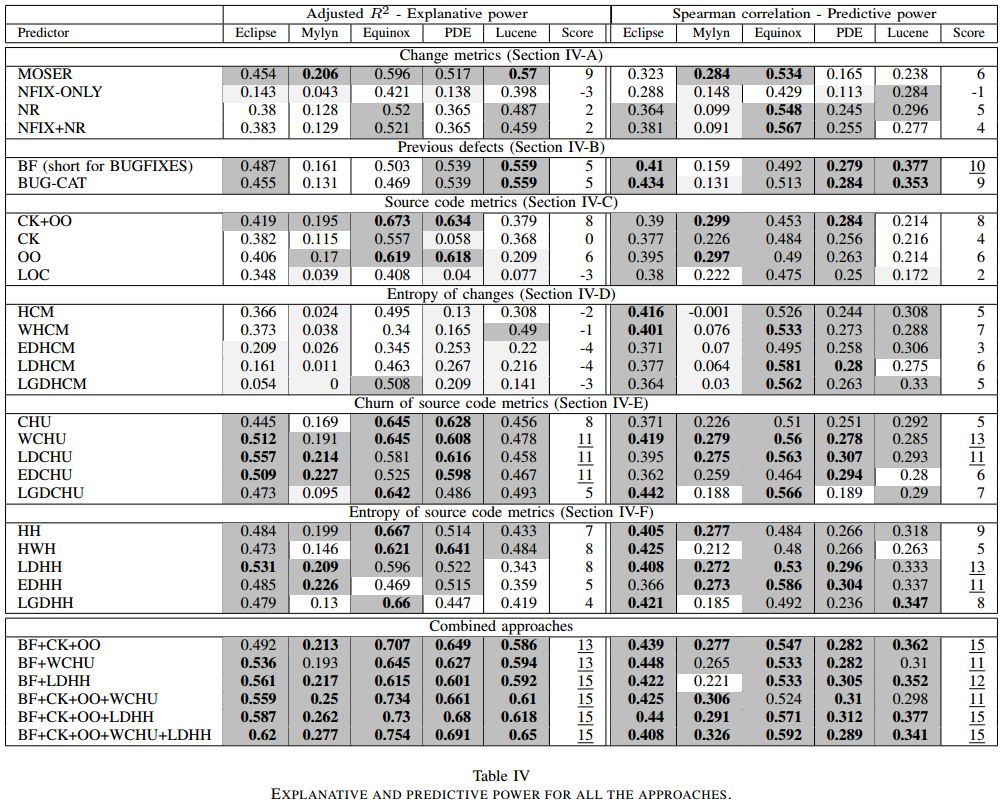
\includegraphics[width=15cm]{results.png}
    \label{fig:B}
\end{figure*}
\begin{itemize}
    \item \underline{Motivation}: The driving scenario is resource allocation: Time and manpower being finite resources, it makes sense to assign personnel and/or resources to areas of a software system with a higher probable quantity of bugs. They want to make it more automated so that it takes less man power.
    \item \underline{Related Work}: To tackle there were many approaches suggested code metrics (lines of code, complexity), process metrics (number of changes, recent activity) or previous defects. Relative code churn was a better predictor than absolute churn. The bug-introducing changes are identified from the SCM logs.  Comparative study among process metrics, system metrics, defect information related and bi-weekly models of each system version if new metrics need to be computed. Entropy was compared to amount of changes and the amount of previous bugs. Chidamber and Kemerer (CK) metrics suite, McCabe’s cyclomatic complexity, Briand’s coupling metrics, code metrics, dependencies between binaries, cohesion measurement based on LSI.
    \item \underline{Patterns}: Predictions at the package-level are less helpful since packages are significantly larger. Package-level information can be derived from class-level information, while the opposite is not true. They used PCA, built regression model. Approaches based on churn and entropy of source code metrics have good and stable explanative and predictive power, better than all the other applied approaches. Using the source code metrics, CK+OO to predict bugs has several advantages: They are lightweight to compute, have good explanative and predictive power and do not require historical information.
    \item \underline{Results}: Please refer Table IV.
    \item \underline{Datasets used} : Six open-source systems: FreeBSD, NetBSD, OpenBSD, KDE, KOffice, and PostgreSQL. Apache, PostgreSQL, Subversion, Mozilla, JEdit, Columba, and Eclipse. Datasets publicly available here\footnote{http://bug.inf.usi.ch}.
\end{itemize}

\subsubsection{\textbf{Conclusion and improvement}}

Using the CK and the OO metric sets together is preferable than using them in isolation, as the performances are more stable across case studies. Bug prediction approaches based on a single metric are not stable over the case studies. The best weighting for past metrics is the linear one. Using string matching on versioning system comments, without validating it on the bug database, decreases the accuracy of bug prediction. Combining bugs and OO metrics improves predictive power. There are scopes of improvement in following ways:
\begin{itemize}
    \item Set of bugs which are linked to commit comments is not a fair representation of the full population of bugs. Need to have better sampling technique.
    \item Considerable fraction of problem reports marked as bugs in Bugzilla (according to their severity) are indeed "non bugs". Need an automated technique to find bugs or not bugs.
\end{itemize}

\subsection{\textbf{A general software defect-proneness prediction framework~\cite{song2011general}}}
\subsubsection{\textbf{Keywords}}
\begin{itemize}
    \item \underline{InfoGain}: The expected information gain is the change in information entropy {H} from a prior state to a state that takes some information.
    \item \underline{Forward selection}:  It starts from an empty set and evaluates each attribute individually to find the best single attribute. It then tries each of the remaining attributes in conjunction with the best to find the best pair of attributes. In the next iteration each of the remaining attributes are tried in conjunction with the best pair to find the best group of three attributes. 
    \item \underline{Backward elimination}: It starts with the whole set of attributes, and eliminates one attribute in each iteration until no single attribute elimination improves the evaluation of the subset.
    \item \underline{Wilcoxon signed-rank test}: It is a non-parametric statistical hypothesis test used when comparing two related samples, matched samples, or repeated measurements on a single sample to assess whether their population mean ranks differ. It can be used as an alternative to the paired Student's t-test, t-test for matched pairs, or the t-test for dependent samples when the population cannot be assumed to be normally distributed.
\end{itemize}

\subsubsection{\textbf{Key Ideas}}
\begin{itemize}
    \item \underline{Motivation}: Different learning schemes are needed for different data sets (i.e. no scheme dominates), that small details in conducting how evaluations are conducted can completely reverse findings and lastly that their proposed framework is more effective, and less prone to bias than previous approaches.
    \item \underline{Related Work}: Capture-recapture (CR) models and detection profile methods (DPM) to estimate the number of defects remaining in software systems with inspection data and process quality data. Association rule mining algorithms reveal software defect associations. Other work classifies software components as defect-prone and non-defect-prone by means of metric-based classification. Their work is mostly inspired by the work done by Menzies et al.~\cite{menzies2007data}. They compared Rule Induction and Naive Bayes to predict software components containing defects.
    \item \underline{Patterns}: The framework should consist of two components: (i) scheme evaluation and (ii) defect prediction. Scheme evaluation will evaluate the machine learning algorithm (which performs better with respect to historical data) before using it for defect prediction. At the first stage, attribute selection is needed that can be categorized as either filters or wrappers and only used on the training set. There is slight difference between Menzies work and this work. Just the order in which cross validation, attribute selection and wrapping filters are applied. Defect prediction with different learning schemes. In short there are 12 comparisons based learning which includes 2 data preprocessors, two attribute selectors, and three learning schemes.
    \item \underline{Datasets used} : The public NASA MDP repository, which was also used by Menzies et al. What’s more, the AR data from the PROMISE repository\footnote{4. http://promise.site.uottowa.ca/SERepository} was also used. Thus there are 17 data sets in total, 13 from NASA and the remaining 4 from the PROMISE repository.
\end{itemize}

\subsubsection{\textbf{Conclusion and improvement}}
 They observed that there is a bigger difference between the evaluation performance
and the actual prediction performance in Menzies et al. study than with their framework. This means that the results reported by Menzies et al. are over optimistic. They contend that their framework is less biased and more capable of yielding results closer to the ‘true’ answer. Moreover, their framework is more
stable. There are scopes of improvement in following ways:
\begin{itemize}
    \item They should report the results by better statistical tests like scott-knot test. 
    \item Data preprocessor/attribute selector can play different roles and they only reported the results with only couple of options.
    \item They surely reported results with 3 different learners, but as they stated these can be quite learner biased. We will need to run many different learners for different datasets.
\end{itemize}

\subsection{\textbf{A systematic literature review on fault prediction performance in software engineering~\cite{hall2012systematic}}}
\subsubsection{\textbf{Keywords}}
\begin{itemize}
    \item \underline{Systematic Literature Review}: A systematic review is a type of literature review that collects and critically analyzes multiple research studies or papers.
    \item \underline{Mean Standard Error}: The MSE is the standard deviation of the sample-mean's estimate of a population mean.
    \item \underline{Area Under Curve}: The area under a curve between two points can be found by doing a definite integral between the two points. To find the area under the curve y = f(x) between x = a and x = b, integrate y = f(x) between the limits of a and b.
    \item \underline{Receiver operating characteristic Curve}: A graphical plot of the sensitivity (or pd) vs. 1 – specificity (or pf) for a binary classification system where its discrimination threshold is varied
\end{itemize}

\subsubsection{\textbf{Key Ideas}}
\begin{itemize}
    \item \underline{Motivation} : Context is important in fault prediction modeling as it can affect the performance of models in a particular context and the transferability of models between contexts. There are a range of independent variables that have been used in fault prediction models. Fault prediction models are based on a wide variety of both machine learning and regression model techniques. Currently the impact context have on transferability of models, the impact individual independent variables have on model performance and the impact modelling technique has on model performance is not clear. This makes it difficult for model builders to make effective technique selections. Hall et al. aims to present a synthesis of current knowledge on the impact of context, independent variables and model techniques on model performance. 
    \item \underline{Sampling Procedures}: A set of 208 studies performed addressing fault prediction in software engineering from January 2000 to December 2010. They defined various criteria to come up with those papers that can be of utmost importance. They defined the paper's inclusion and exclusion criteria, Paper selection and validation process, Prediction criteria, context criteria, model building criteria, data criteria.
    \item \underline{Patterns}: The context of models has not been studied extensively in the set of studies they analysed. This is a significant gap in current knowledge as it means we currently do not know what context factors influence how well a model will transfer to other systems. Models using only static code metrics (typically complexity-based) perform relatively poorly. Model performance does not seem to improve by combining these metrics with OO metrics. Models seem to perform better using only OO metrics. The use of process data is not particularly related to good predictive performance. Analysis suggests that studies using Support Vector Machine (SVM) techniques perform less well. These may be underperforming as they require parameter optimization. Models based on C4.5 seem to underperform if they have imbalanced data. Naive Bayes and Logistic regression, in particular, seem to be the techniques used in models that are performing relatively well. 
    \item \underline{Anti-Patterns}: Prediction shouldn't be performed if data quality is poor. Good data quality is important for prediction. Data should not be imbalanced. There is no one best way to measure the performance of a model. Performance comparison across studies is only possible if studies report a set of uniform measures. Companies developing non-critical systems may want to prioritise their fault finding effort only on the most severe faults.
\end{itemize}

\subsubsection{\textbf{Conclusion and improvement}}
Their results suggest that models which perform well tend to be built in a context where the systems are large. We found no evidence that the maturity of systems or
the language used is related to predictive performance. Overall they conclude that many good fault prediction studies have been reported in software engineering.
There are scopes of improvement in following ways:
\begin{itemize}
    \item We need more studies which are based on a reliable methodology and which consistently report the context in which models are built and the methodology used to build them.
    \item A larger set of such studies will enable reliable cross-study metaanalysis of model performance. It will also give practitioners the confidence to appropriately select and apply models to their systems.
    \item Cross project defect/fault prediction can be done too, where privacy of data is of concern.
    \item Hyperparameter optimization of learners should be done.
    \item For imbalanced dataset, SMOTE~\cite{chawla2002smote} could be used.
\end{itemize}

\section{Survey After 2012}
\label{after}
The following papers were comprises after Hall et al.~\cite{hall2012systematic}
published on the Systematic literature review on fault prediction performance in Software Engineering in 2012. For each paper, we  provide a bullet point format, defining keywords described by each author, summarizing selected ideas presented in each paper, and finally, the conclusion and describing what can be made to improve the results.

\subsection{\textbf{Software fault prediction metrics: A systematic literature review~\cite{radjenovic2013software}}}
\subsubsection{\textbf{Keywords}}
\begin{itemize}
    \item \underline{Software metric}: A software metric is a standard of measure of a degree to which a software system or process possesses some property.
    \item \underline{MOOD metrics suite}: The MOOD metrics suite includes 6 metrics: Method Hiding Factor, Attribute Hiding Factor, Method Inheritance Factor, Attribute Inheritance Factor, Polymorphism Factor, and Coupling Factor.
    \item \underline{CK metrics suite}: The CK metrics suite includes 6 metrics: Weighted Method Class, Depth of Inheritance tree, Number of children, Coupling between Object Classes, Response for a class, and Lack of cohesion in Methods.
\end{itemize}

\subsubsection{\textbf{Key Ideas}}
\begin{itemize}
    \item \underline{Motivation}: In software fault prediction many software metrics have been proposed. Many of them have been validated only in a small number of studies. Some of them have been proposed but never used. Contradictory results across studies have been reported. Even withing a single study, different results have been obtained when different environments or methods have been used. The aim of the authors were to depict current state-of-the-art metrics in software fault prediction.
    \item \underline{Related Work}: A systematic review of software fault prediction studies was performed by Catal et al~\cite{catal2009systematic}. In 2012, a review similar in design to Catal et al, but more comprehensive in terms of the number of included studies and analyses, was published by Hall et al~\cite{hall2012systematic}. In the review, papers on software fault prediction were included focusing again on empirical studies. This paper is different from the above reviews in both the aim and scope of selected  studies. The objective of this review are to asses primary studies that empirically validate software metrics in software fault prediction and to assess metrics used in these studies according to several properties.
    \item \underline{Patterns}: Validations should be performed in the most realistic environment possible in order to acquire results relevant for the industry. In realistic environments, faults are fairly random and data sets are highly unbalanced (few faults, many correct modules). The number of faults and their distribution between two releases can be significantly different. Validation techniques, like a 10-fold cross-validation, 2/3 for training and 1/3 for testing, do not take into account all the factors that real environment validation does. Only validation where models are trained on release i and evaluated on i+1, can determine the impact of all these, and other unpredictable factors, of the environment.
    \item \underline{Sampling Procedures}: A set of 106 primary studies evaluating software metrics performed addressing fault prediction in software engineering. They defined various criteria to come up with those papers that can be of utmost importance. They defined the paper's inclusion and exclusion criteria, Paper selection and validation process, Prediction criteria, context criteria, model building criteria, data criteria.
\end{itemize}

\subsubsection{\textbf{Conclusion and improvement}}
Object-oriented metrics (49\%) were used nearly twice as often compared to traditional source code metrics (27\%) or process metrics (24\%). Chidamber and Kemerer's (CK) objected-oriented metrics were most frequently used. According to the selected studies there are significant differences between the metrics used in fault prediction performance. Objected-oriented and process metrics have been reported to be more successful in finding faults faults compared to any traditional size and complexity metrics.
There are scopes of improvement in following ways:
\begin{itemize}
    \item More studies should be performed on large industrial software systems to find metrics more relevant for the industry and to answer the question as to which metrics should be used in a given context.
\end{itemize}

\subsection{\textbf{Researcher Bias: The Use of Machine Learning in Software Defect Prediction~\cite{shepperd2014researcher}}}
\subsubsection{\textbf{Keywords}}
\begin{itemize}
    \item \underline{Software defect prediction}: Software Defect Prediction (SDP) is one of the most assisting activities of the Testing Phase of SDLC. It identifies the modules that are defect prone and require extensive testing. This way, the testing resources can be used efficiently without violating the constraints.
    \item \underline{Meta-Analysis}: In statistics, meta-analysis comprises statistical methods for contrasting and combining results from different studies, in the hope of identifying patterns among study results, sources of disagreement among those results, or other interesting relationships that may come to light in the context of multiple studies.
    \item \underline{Researcher Bias}: Research bias, also called experimenter bias, is a process where the scientists performing the research influence the results, in order to portray a certain outcome.
    \item \underline{Matthews correlation coefficient}: MCC is used in machine learning as a measure of the quality of binary (two class) classifications.
\end{itemize}

\subsubsection{\textbf{Key Ideas}}
\begin{itemize}
    \item \underline{Motivation} : The ability to predict defect-prone software components would be valuable. Consequently, there have been many empirical studies to evaluate the performance of different techniques endeavouring to accomplish this effectively. However, no one technique dominates and so designing a reliable defect prediction model remains problematic. They seek to make sense of the many conflicting experimental results and understand which factors have the largest effect on predictive performance.
    \item \underline{Related Work}: There has been very substantial research effort put into software defect prediction. However, a consensus on what are the best prediction techniques, even for a specific context, remains elusive. This paper finds considerable diversity as to what form of classifier technique should be used and what inputs or metrics work best. In addition, in order to facilitate generalisation, researchers are using an increasing number of different defect data sets for empirical validation. Unfortunately the situation is somewhat complicated by the use of a wide range of validation schemes. The time is ripe to explore the underlying reasons for this lack of convergence in results hence this paper conducted a meta-analysis. This will provide pointers to the most effective way forward for future software defect prediction research.
    \item \underline{Sampling Procedures}: They conducted a meta-analysis of all relevant, high quality primary studies of defect prediction to determine what factors influence predictive performance. This is based on 42 primary studies that satisfy our inclusion criteria that collectively report 600 sets of empirical prediction results.
    \item \underline{Patterns}: There is no uniformity amongst researchers as to how classification performance should be reported. This lack of uniformity has necessitated them to reverse engineer a common performance statistic (the Matthews correlation coefficient (MCC). By reverse engineering a common response variable, they built a random effects ANOVA model to examine the relative contribution of four model building factors (classifier, data set, input metrics and researcher group) to model prediction performance. The number of observations of the correlation coefficient is close to zero or even negative. This reveals that many classifiers are performing extremely poorly, since zero indicates no relationship at all and could therefore be achieved through guessing. A negative value means the prediction would be improved by adding an inverter. Moreover, the modal value lies in the range of 0.3-0.4 which hardly engenders a great deal of confidence in terms of their practical use.
\end{itemize}

\subsubsection{\textbf{Conclusion and improvement}}
The variability due to the choice of classifier is extremely small. The variability due to the groups of researchers (Researcher Group) could be seen as twenty five times higher. There are differing levels of expertise between researcher groups and second, there is the widespread problem of researcher bias.
There are scopes of improvement in following ways:
\begin{itemize}
    \item Improving communication and documentation will help protect against the other things which researcher groups are doing, i.e. the unwritten setup is just as important as that which is documented.
    \item Joint comparative empirical studies of defect prediction
between research centres such that researcher
groups do not have to be expert in all classifier
learning techniques.
\end{itemize}

\subsection{\textbf{Revisiting the impact of classification techniques on the performance of defect prediction models~\cite{ghotra2015revisiting}}}
\subsubsection{\textbf{Keywords}}
\begin{itemize}
    \item \underline{MARS}: Multivariate Adaptive Regression Splines is a non-parametric regression technique and can be seen as an extension of linear models that automatically models nonlinearities and interactions between variables.
    \item \underline{LMT}: logistic model tree (LMT) is a classification model with an associated supervised training algorithm that combines logistic regression (LR) and decision tree learning.
    \item \underline{Expectation Maximization}: An EM algorithm is an iterative method for finding maximum likelihood or maximum a posteriori (MAP) estimates of parameters in statistical models, where the model depends on unobserved latent variables.
    \item \underline{SMO}: Sequential minimal optimization is an algorithm for solving the quadratic programming (QP) problem that arises during the training of support vector machines.
\end{itemize}

\subsubsection{\textbf{Key Ideas}}
\begin{itemize}
    \item \underline{Motivation}: Their results suggest that some classification techniques tend to produce defect prediction models that outperform others on contrary to earlier research which stated the classification techniques didnt matter.
    \item \underline{Patterns}: Logistic regression and linear regression, Multivariate Adaptive Regression Splines, Personalized Change Classification, and Logistic Model Trees. Ensemble methods that combine different machine learning techniques have also been explored. Lessmann et al.~\cite{lessmann2008benchmarking} conducted a study comparing the performance of 22 different classification techniques on the NASA corpus. Their results show that the performance of 17 of the 22 classification techniques are statistically indistinguishable from each other. Table I shows different kinds of classification techniques being studied.
    \begin{figure}[!htbp]
     \centering
    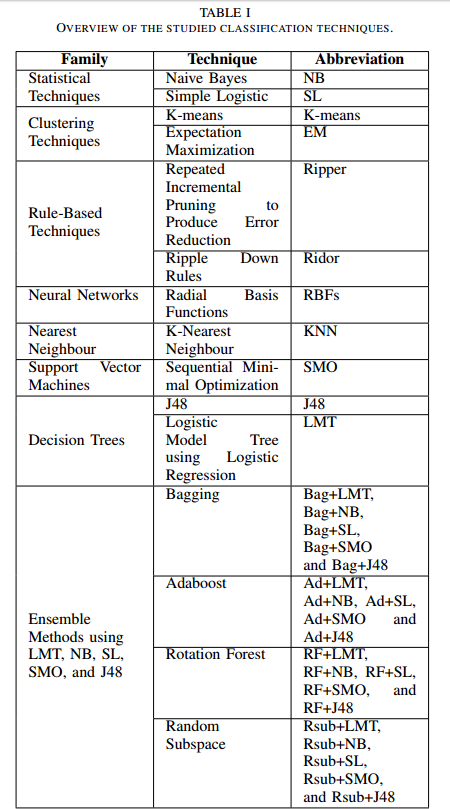
\includegraphics[width=\linewidth]{learners.png}
  \label{fig:2c}
\end{figure}
    \item \underline{Assessment}: To compare the performance of defect prediction models, they used the Area Under the receiver operating characteristic Curve (AUC), which plots the false positive rate against the true positive rate. They ran the Scott-Knott test to group classification techniques into statistically distinct ranks.
\end{itemize}

\subsubsection{\textbf{Conclusion and improvement}}
Ensemble techniques (i.e., RF+a base learner), decision trees
(i.e., LMT), statistical techniques (i.e., Simple Logistic and
Naive Bayes), neural networks (i.e., RBFs), and nearest neighbour
(i.e., KNN) outperformed models trained using rule-based
techniques (i.e., Ripper and Ridor), clustering techniques (i.e.,
K-means and EM) and SVM (i.e., SMO).
There are scopes of improvement in following ways:
\begin{itemize}
    \item They studied 2 datasets which have different predictor metrics, this difference might be the reason for their results. They should have unified the metrics properly and then have come out for a conclusion. 
    \item This kind of study also gives rise to cross project defect prediction and unifying the predictor metrics.
    \item Since they tested on so many different techniques, they can now work on hyperparameter optimization of learners, to come up with other explanations.
\end{itemize}

\subsection{\textbf{Automated Parameter Optimization of Classification Techniques for Defect Prediction Models~\cite{tantithamthavorn2016automated}}}
\begin{figure*}[!htbp]
    \centering
    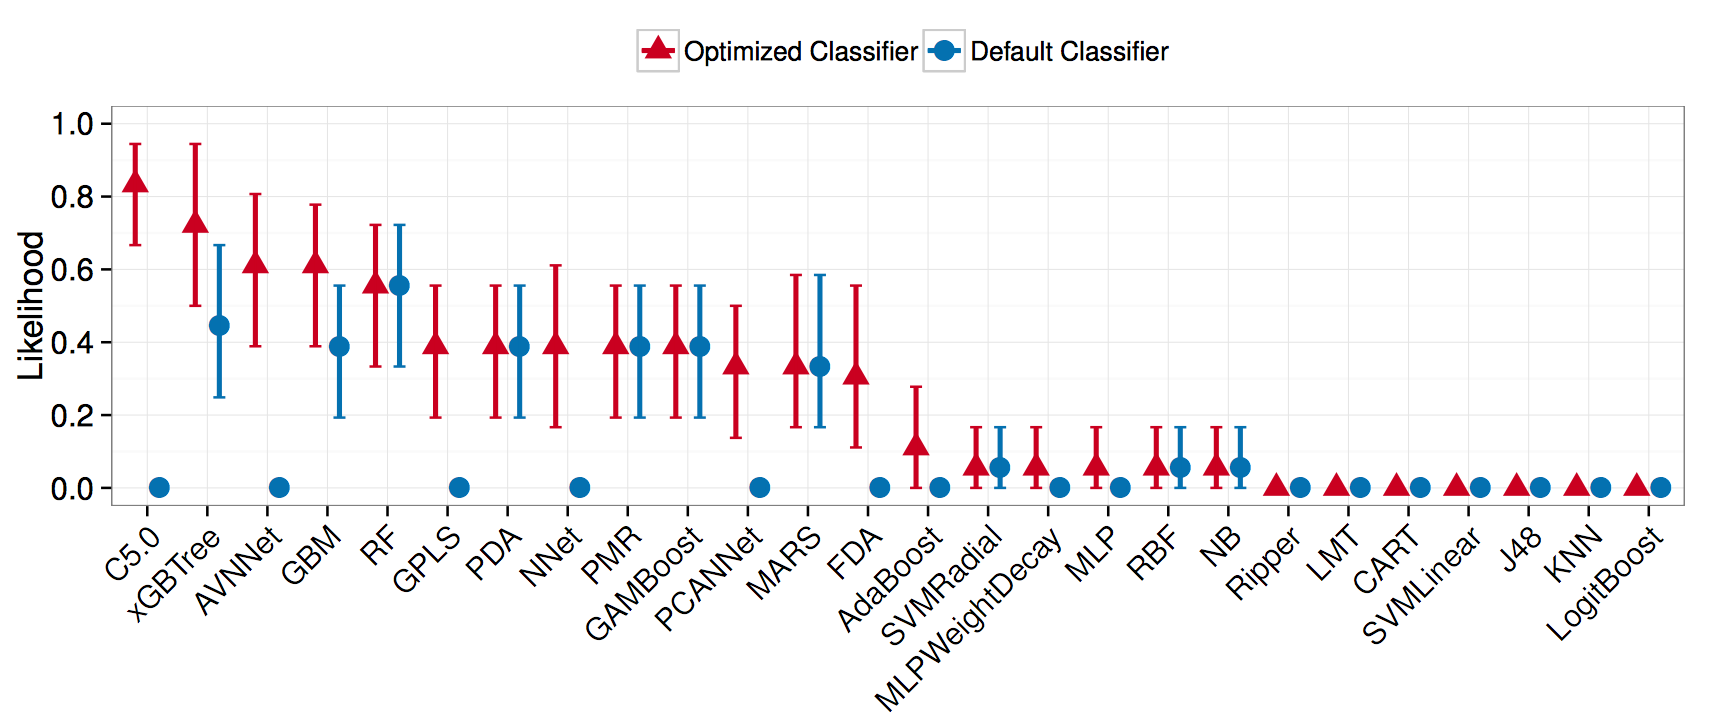
\includegraphics[width=\linewidth]{Read_8.png}
    \caption{The likelihood of each technique appearing in the top Scott-Knott rank. Circle dots and
triangle dots indicate the median likelihood, while the error bars indicate the 95\% confidence interval of the
likelihood of the bootstrap analysis. A likelihood of 80\% indicates that a classification technique appears at
the top-rank for 80\% of the studied datasets}
    \label{fig:c}
\end{figure*}
\subsubsection{\textbf{Keywords}}
\begin{itemize}
    \item \underline{Experimental Design}: The design of experiments (DOE, DOX, or experimental design) is the design of any task that aims to describe or explain the variation of information under conditions that are hypothesized to reflect the variation.
    \item \underline{Classification Techniques}: In machine learning and statistics, classification is the problem of identifying to which of a set of categories (sub-populations) a new observation belongs, on the basis of a training set of data containing observations (or instances) whose category membership is known. Eg. Naive Bayes classifier, Logistic regression etc.
    \item \underline{Parameter Optimization}: In the context of machine learning, parameter optimization or model selection is the problem of choosing a set of parameters for a learning algorithm, usually with the goal of optimizing a measure of the algorithm's performance on an independent data set. Often cross-validation is used to estimate this generalization performance.
\end{itemize}

\subsubsection{\textbf{Key Ideas}}

\begin{itemize}
    \item \underline{Motivation}: Defect prediction models are classifiers that are trained to identify defect-prone software modules. Such classifiers have configurable parameters that control their characteristics (e.g., the number of trees in a random forest classifier). Recent studies show that these classifiers may underperform due to the use of suboptimal default parameter settings. However, it is impractical to assess all of the possible settings in the parameter spaces. This paper investigates the performance of defect prediction models where Caret~\cite{kuhn2015caret} — an automated parameter optimization technique — has been applied.
    \item \underline{Related Work}: Recent research~\cite{fu2016tuning,agrawal2016wrong} has raised concerns about parameter settings of different data miners. Some other studies shows the effect of parameter settings of classification techniques when applied to defect prediction models. For example, Koru et al.~\cite{koru2005investigation} and Mende et al.~\cite{mende2010replication} point out that selecting different parameter settings can impact the performance of defect models. Jiang et al.~\cite{jiang2008can} and Tosun et al.~\cite{tosun2009reducing} also point out that the default parameter settings of research toolkits (e.g., R, Weka, Scikit-learn, MATLAB) are suboptimal. Although prior work suggests that defect prediction models may underperform if they are trained using suboptimal parameter settings, parameters are often left at their default values. Recent research voices concerns about the stability of performance estimates that are obtained from classification techniques when applied to defect prediction models. For example, Menzies et al.~\cite{menzies2012special} and Mittas et al.~\cite{mittas2013ranking} argue that unstable classification techniques can make replication of defect prediction studies more difficult. Like any form of classifier optimization, automated parameter optimization may increase the risk of overfitting, i.e., producing a classifier that is too specialized for the data from which it was trained to apply to other datasets. 
    \item \underline{Informative Visualization}: The figure~\ref{fig:c} summarises the results.
\end{itemize}

\subsubsection{\textbf{Conclusion and improvement}}
C5.0 boosting tends to yield top-performing defect prediction models more frequently than the other studied classification techniques. Automated parameter optimization increases the likelihood of appearing in the top Scott-Knott rank by as much as 83\%. Automated parameter optimization increases the likelihood of 11 of the studied 26 classification techniques by as much as 83\% (i.e., C5.0 boosting). This suggests that automated parameter optimization can substantially shift the ranking of classification techniques. Since automated parameter optimization techniques like Caret yield substantially benefits in terms of performance improvement and stability, while incurring a manageable additional computational cost, this paper suggests researchers should be included in future defect prediction studies.
There are scopes of improvement in following ways:
\begin{itemize}
    \item Since computational cost is high, we can go for much simple optimizers like differential evolution~\cite{storn1997differential}.
\end{itemize}

\section{Discussion and Conclusion}
\label{conclusion}
After such an extensive study, we find some take away points. They are mentioned below.
\begin{itemize}
    \item The combined or socio-technical models for any of the evaluation metrics can give a good prediction model.
    \item Using the CK and the OO metric sets together is preferable than using them in isolation.
    \item Random Forest, naive bayes, simple logistic, decision trees, and nearest neighbors perform better in defect prediction.
    \item Sometimes the data is imbalanced and we should balance the classes.
    \item Tuning the parameters of classification gives enormous difference in performance, so tuning can not be neglected.
    \item Cross project defect prediction should be our next concern.
\end{itemize}

\ifCLASSOPTIONcaptionsoff
  \newpage
\fi

\balance

\bibliographystyle{abbrv}
\medskip
\bibliography{ref}

\end{document}


